% Created by tikzDevice version 0.12 on 2019-05-24 17:17:27
% !TEX encoding = UTF-8 Unicode
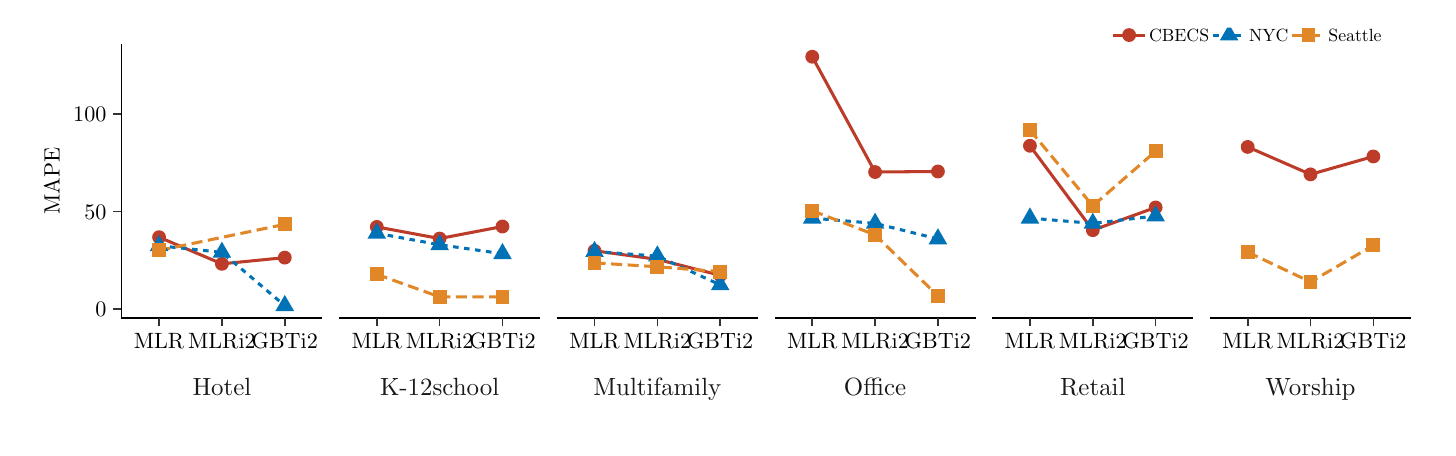
\begin{tikzpicture}[x=1pt,y=1pt]
\definecolor{fillColor}{RGB}{255,255,255}
\path[use as bounding box,fill=fillColor,fill opacity=0.00] (0,0) rectangle (505.89,144.54);
\begin{scope}
\path[clip] (  0.00,  0.00) rectangle (505.89,144.54);
\definecolor{drawColor}{RGB}{255,255,255}
\definecolor{fillColor}{RGB}{255,255,255}

\path[draw=drawColor,line width= 0.6pt,line join=round,line cap=round,fill=fillColor] (  0.00,  0.00) rectangle (505.89,144.54);
\end{scope}
\begin{scope}
\path[clip] ( 33.85, 39.60) rectangle (106.52,138.54);
\definecolor{fillColor}{RGB}{255,255,255}

\path[fill=fillColor] ( 33.85, 39.60) rectangle (106.52,138.54);
\definecolor{drawColor}{RGB}{188,60,41}

\path[draw=drawColor,line width= 1.1pt,line join=round] ( 47.48, 68.83) --
	( 70.19, 59.20) --
	( 92.90, 61.45);
\definecolor{drawColor}{RGB}{0,114,181}

\path[draw=drawColor,line width= 1.1pt,dash pattern=on 2pt off 2pt ,line join=round] ( 47.48, 65.74) --
	( 70.19, 63.35) --
	( 92.90, 44.09);
\definecolor{drawColor}{RGB}{225,135,39}

\path[draw=drawColor,line width= 1.1pt,dash pattern=on 4pt off 2pt ,line join=round] ( 47.48, 64.05) --
	( 92.90, 73.47);
\definecolor{fillColor}{RGB}{188,60,41}

\path[fill=fillColor] ( 47.48, 68.83) circle (  2.50);

\path[fill=fillColor] ( 70.19, 59.20) circle (  2.50);

\path[fill=fillColor] ( 92.90, 61.45) circle (  2.50);
\definecolor{fillColor}{RGB}{0,114,181}

\path[fill=fillColor] ( 47.48, 69.62) --
	( 50.84, 63.80) --
	( 44.11, 63.80) --
	cycle;

\path[fill=fillColor] ( 70.19, 67.23) --
	( 73.55, 61.41) --
	( 66.82, 61.41) --
	cycle;

\path[fill=fillColor] ( 92.90, 47.98) --
	( 96.26, 42.15) --
	( 89.53, 42.15) --
	cycle;
\definecolor{fillColor}{RGB}{225,135,39}

\path[fill=fillColor] ( 44.98, 61.55) --
	( 49.97, 61.55) --
	( 49.97, 66.55) --
	( 44.98, 66.55) --
	cycle;

\path[fill=fillColor] ( 90.40, 70.97) --
	( 95.40, 70.97) --
	( 95.40, 75.97) --
	( 90.40, 75.97) --
	cycle;
\end{scope}
\begin{scope}
\path[clip] (112.52, 39.60) rectangle (185.20,138.54);
\definecolor{fillColor}{RGB}{255,255,255}

\path[fill=fillColor] (112.52, 39.60) rectangle (185.20,138.54);
\definecolor{drawColor}{RGB}{188,60,41}

\path[draw=drawColor,line width= 1.1pt,line join=round] (126.15, 72.55) --
	(148.86, 68.34) --
	(171.57, 72.69);
\definecolor{drawColor}{RGB}{0,114,181}

\path[draw=drawColor,line width= 1.1pt,dash pattern=on 2pt off 2pt ,line join=round] (126.15, 70.24) --
	(148.86, 66.09) --
	(171.57, 62.86);
\definecolor{drawColor}{RGB}{225,135,39}

\path[draw=drawColor,line width= 1.1pt,dash pattern=on 4pt off 2pt ,line join=round] (126.15, 55.41) --
	(148.86, 47.26) --
	(171.57, 47.26);
\definecolor{fillColor}{RGB}{188,60,41}

\path[fill=fillColor] (126.15, 72.55) circle (  2.50);

\path[fill=fillColor] (148.86, 68.34) circle (  2.50);

\path[fill=fillColor] (171.57, 72.69) circle (  2.50);
\definecolor{fillColor}{RGB}{0,114,181}

\path[fill=fillColor] (126.15, 74.12) --
	(129.51, 68.29) --
	(122.79, 68.29) --
	cycle;

\path[fill=fillColor] (148.86, 69.97) --
	(152.22, 64.15) --
	(145.50, 64.15) --
	cycle;

\path[fill=fillColor] (171.57, 66.74) --
	(174.93, 60.91) --
	(168.21, 60.91) --
	cycle;
\definecolor{fillColor}{RGB}{225,135,39}

\path[fill=fillColor] (123.65, 52.91) --
	(128.65, 52.91) --
	(128.65, 57.91) --
	(123.65, 57.91) --
	cycle;

\path[fill=fillColor] (146.36, 44.76) --
	(151.36, 44.76) --
	(151.36, 49.75) --
	(146.36, 49.75) --
	cycle;

\path[fill=fillColor] (169.07, 44.76) --
	(174.07, 44.76) --
	(174.07, 49.75) --
	(169.07, 49.75) --
	cycle;
\end{scope}
\begin{scope}
\path[clip] (191.20, 39.60) rectangle (263.87,138.54);
\definecolor{fillColor}{RGB}{255,255,255}

\path[fill=fillColor] (191.20, 39.60) rectangle (263.87,138.54);
\definecolor{drawColor}{RGB}{188,60,41}

\path[draw=drawColor,line width= 1.1pt,line join=round] (204.82, 63.91) --
	(227.53, 60.82) --
	(250.24, 55.06);
\definecolor{drawColor}{RGB}{0,114,181}

\path[draw=drawColor,line width= 1.1pt,dash pattern=on 2pt off 2pt ,line join=round] (204.82, 63.63) --
	(227.53, 62.01) --
	(250.24, 51.61);
\definecolor{drawColor}{RGB}{225,135,39}

\path[draw=drawColor,line width= 1.1pt,dash pattern=on 4pt off 2pt ,line join=round] (204.82, 59.55) --
	(227.53, 58.15) --
	(250.24, 56.39);
\definecolor{fillColor}{RGB}{188,60,41}

\path[fill=fillColor] (204.82, 63.91) circle (  2.50);

\path[fill=fillColor] (227.53, 60.82) circle (  2.50);

\path[fill=fillColor] (250.24, 55.06) circle (  2.50);
\definecolor{fillColor}{RGB}{0,114,181}

\path[fill=fillColor] (204.82, 67.51) --
	(208.19, 61.69) --
	(201.46, 61.69) --
	cycle;

\path[fill=fillColor] (227.53, 65.90) --
	(230.90, 60.07) --
	(224.17, 60.07) --
	cycle;

\path[fill=fillColor] (250.24, 55.50) --
	(253.61, 49.67) --
	(246.88, 49.67) --
	cycle;
\definecolor{fillColor}{RGB}{225,135,39}

\path[fill=fillColor] (202.33, 57.06) --
	(207.32, 57.06) --
	(207.32, 62.05) --
	(202.33, 62.05) --
	cycle;

\path[fill=fillColor] (225.04, 55.65) --
	(230.03, 55.65) --
	(230.03, 60.65) --
	(225.04, 60.65) --
	cycle;

\path[fill=fillColor] (247.75, 53.89) --
	(252.74, 53.89) --
	(252.74, 58.89) --
	(247.75, 58.89) --
	cycle;
\end{scope}
\begin{scope}
\path[clip] (269.87, 39.60) rectangle (342.54,138.54);
\definecolor{fillColor}{RGB}{255,255,255}

\path[fill=fillColor] (269.87, 39.60) rectangle (342.54,138.54);
\definecolor{drawColor}{RGB}{188,60,41}

\path[draw=drawColor,line width= 1.1pt,line join=round] (283.50,134.04) --
	(306.21, 92.37) --
	(328.92, 92.58);
\definecolor{drawColor}{RGB}{0,114,181}

\path[draw=drawColor,line width= 1.1pt,dash pattern=on 2pt off 2pt ,line join=round] (283.50, 75.72) --
	(306.21, 73.82) --
	(328.92, 68.20);
\definecolor{drawColor}{RGB}{225,135,39}

\path[draw=drawColor,line width= 1.1pt,dash pattern=on 4pt off 2pt ,line join=round] (283.50, 78.39) --
	(306.21, 69.67) --
	(328.92, 47.61);
\definecolor{fillColor}{RGB}{188,60,41}

\path[fill=fillColor] (283.50,134.04) circle (  2.50);

\path[fill=fillColor] (306.21, 92.37) circle (  2.50);

\path[fill=fillColor] (328.92, 92.58) circle (  2.50);
\definecolor{fillColor}{RGB}{0,114,181}

\path[fill=fillColor] (283.50, 79.60) --
	(286.86, 73.77) --
	(280.13, 73.77) --
	cycle;

\path[fill=fillColor] (306.21, 77.70) --
	(309.57, 71.88) --
	(302.84, 71.88) --
	cycle;

\path[fill=fillColor] (328.92, 72.08) --
	(332.28, 66.26) --
	(325.55, 66.26) --
	cycle;
\definecolor{fillColor}{RGB}{225,135,39}

\path[fill=fillColor] (281.00, 75.89) --
	(285.99, 75.89) --
	(285.99, 80.88) --
	(281.00, 80.88) --
	cycle;

\path[fill=fillColor] (303.71, 67.18) --
	(308.70, 67.18) --
	(308.70, 72.17) --
	(303.71, 72.17) --
	cycle;

\path[fill=fillColor] (326.42, 45.11) --
	(331.42, 45.11) --
	(331.42, 50.10) --
	(326.42, 50.10) --
	cycle;
\end{scope}
\begin{scope}
\path[clip] (348.54, 39.60) rectangle (421.22,138.54);
\definecolor{fillColor}{RGB}{255,255,255}

\path[fill=fillColor] (348.54, 39.60) rectangle (421.22,138.54);
\definecolor{drawColor}{RGB}{188,60,41}

\path[draw=drawColor,line width= 1.1pt,line join=round] (362.17,101.86) --
	(384.88, 71.36) --
	(407.59, 79.58);
\definecolor{drawColor}{RGB}{0,114,181}

\path[draw=drawColor,line width= 1.1pt,dash pattern=on 2pt off 2pt ,line join=round] (362.17, 75.72) --
	(384.88, 73.82) --
	(407.59, 76.49);
\definecolor{drawColor}{RGB}{225,135,39}

\path[draw=drawColor,line width= 1.1pt,dash pattern=on 4pt off 2pt ,line join=round] (362.17,107.55) --
	(384.88, 80.14) --
	(407.59, 99.89);
\definecolor{fillColor}{RGB}{188,60,41}

\path[fill=fillColor] (362.17,101.86) circle (  2.50);

\path[fill=fillColor] (384.88, 71.36) circle (  2.50);

\path[fill=fillColor] (407.59, 79.58) circle (  2.50);
\definecolor{fillColor}{RGB}{0,114,181}

\path[fill=fillColor] (362.17, 79.60) --
	(365.53, 73.77) --
	(358.81, 73.77) --
	cycle;

\path[fill=fillColor] (384.88, 77.70) --
	(388.24, 71.88) --
	(381.52, 71.88) --
	cycle;

\path[fill=fillColor] (407.59, 80.37) --
	(410.95, 74.55) --
	(404.23, 74.55) --
	cycle;
\definecolor{fillColor}{RGB}{225,135,39}

\path[fill=fillColor] (359.67,105.05) --
	(364.67,105.05) --
	(364.67,110.05) --
	(359.67,110.05) --
	cycle;

\path[fill=fillColor] (382.38, 77.65) --
	(387.38, 77.65) --
	(387.38, 82.64) --
	(382.38, 82.64) --
	cycle;

\path[fill=fillColor] (405.09, 97.39) --
	(410.09, 97.39) --
	(410.09,102.39) --
	(405.09,102.39) --
	cycle;
\end{scope}
\begin{scope}
\path[clip] (427.22, 39.60) rectangle (499.89,138.54);
\definecolor{fillColor}{RGB}{255,255,255}

\path[fill=fillColor] (427.22, 39.60) rectangle (499.89,138.54);
\definecolor{drawColor}{RGB}{188,60,41}

\path[draw=drawColor,line width= 1.1pt,line join=round] (440.84,101.44) --
	(463.55, 91.53) --
	(486.26, 97.99);
\definecolor{drawColor}{RGB}{225,135,39}

\path[draw=drawColor,line width= 1.1pt,dash pattern=on 4pt off 2pt ,line join=round] (440.84, 63.42) --
	(463.55, 52.67) --
	(486.26, 65.88);
\definecolor{fillColor}{RGB}{188,60,41}

\path[fill=fillColor] (440.84,101.44) circle (  2.50);

\path[fill=fillColor] (463.55, 91.53) circle (  2.50);

\path[fill=fillColor] (486.26, 97.99) circle (  2.50);
\definecolor{fillColor}{RGB}{225,135,39}

\path[fill=fillColor] (438.35, 60.92) --
	(443.34, 60.92) --
	(443.34, 65.92) --
	(438.35, 65.92) --
	cycle;

\path[fill=fillColor] (461.06, 50.17) --
	(466.05, 50.17) --
	(466.05, 55.16) --
	(461.06, 55.16) --
	cycle;

\path[fill=fillColor] (483.77, 63.38) --
	(488.76, 63.38) --
	(488.76, 68.38) --
	(483.77, 68.38) --
	cycle;
\end{scope}
\begin{scope}
\path[clip] ( 33.85,  6.00) rectangle (106.52, 23.74);
\definecolor{drawColor}{gray}{0.10}

\node[text=drawColor,anchor=base,inner sep=0pt, outer sep=0pt, scale=  0.90] at ( 70.19, 11.77) {Hotel};
\end{scope}
\begin{scope}
\path[clip] (112.52,  6.00) rectangle (185.20, 23.74);
\definecolor{drawColor}{gray}{0.10}

\node[text=drawColor,anchor=base,inner sep=0pt, outer sep=0pt, scale=  0.90] at (148.86, 11.77) {K-12school};
\end{scope}
\begin{scope}
\path[clip] (191.20,  6.00) rectangle (263.87, 23.74);
\definecolor{drawColor}{gray}{0.10}

\node[text=drawColor,anchor=base,inner sep=0pt, outer sep=0pt, scale=  0.90] at (227.53, 11.77) {Multifamily};
\end{scope}
\begin{scope}
\path[clip] (269.87,  6.00) rectangle (342.54, 23.74);
\definecolor{drawColor}{gray}{0.10}

\node[text=drawColor,anchor=base,inner sep=0pt, outer sep=0pt, scale=  0.90] at (306.21, 11.77) {Office};
\end{scope}
\begin{scope}
\path[clip] (348.54,  6.00) rectangle (421.22, 23.74);
\definecolor{drawColor}{gray}{0.10}

\node[text=drawColor,anchor=base,inner sep=0pt, outer sep=0pt, scale=  0.90] at (384.88, 11.77) {Retail};
\end{scope}
\begin{scope}
\path[clip] (427.22,  6.00) rectangle (499.89, 23.74);
\definecolor{drawColor}{gray}{0.10}

\node[text=drawColor,anchor=base,inner sep=0pt, outer sep=0pt, scale=  0.90] at (463.55, 11.77) {Worship};
\end{scope}
\begin{scope}
\path[clip] (  0.00,  0.00) rectangle (505.89,144.54);
\definecolor{drawColor}{RGB}{0,0,0}

\path[draw=drawColor,line width= 0.6pt,line join=round] ( 33.85, 39.60) --
	(106.52, 39.60);
\end{scope}
\begin{scope}
\path[clip] (  0.00,  0.00) rectangle (505.89,144.54);
\definecolor{drawColor}{gray}{0.20}

\path[draw=drawColor,line width= 0.6pt,line join=round] ( 47.48, 36.60) --
	( 47.48, 39.60);

\path[draw=drawColor,line width= 0.6pt,line join=round] ( 70.19, 36.60) --
	( 70.19, 39.60);

\path[draw=drawColor,line width= 0.6pt,line join=round] ( 92.90, 36.60) --
	( 92.90, 39.60);
\end{scope}
\begin{scope}
\path[clip] (  0.00,  0.00) rectangle (505.89,144.54);
\definecolor{drawColor}{RGB}{0,0,0}

\node[text=drawColor,anchor=base,inner sep=0pt, outer sep=0pt, scale=  0.80] at ( 47.48, 28.69) {MLR};

\node[text=drawColor,anchor=base,inner sep=0pt, outer sep=0pt, scale=  0.80] at ( 70.19, 28.69) {MLRi2};

\node[text=drawColor,anchor=base,inner sep=0pt, outer sep=0pt, scale=  0.80] at ( 92.90, 28.69) {GBTi2};
\end{scope}
\begin{scope}
\path[clip] (  0.00,  0.00) rectangle (505.89,144.54);
\definecolor{drawColor}{RGB}{0,0,0}

\path[draw=drawColor,line width= 0.6pt,line join=round] (112.52, 39.60) --
	(185.20, 39.60);
\end{scope}
\begin{scope}
\path[clip] (  0.00,  0.00) rectangle (505.89,144.54);
\definecolor{drawColor}{gray}{0.20}

\path[draw=drawColor,line width= 0.6pt,line join=round] (126.15, 36.60) --
	(126.15, 39.60);

\path[draw=drawColor,line width= 0.6pt,line join=round] (148.86, 36.60) --
	(148.86, 39.60);

\path[draw=drawColor,line width= 0.6pt,line join=round] (171.57, 36.60) --
	(171.57, 39.60);
\end{scope}
\begin{scope}
\path[clip] (  0.00,  0.00) rectangle (505.89,144.54);
\definecolor{drawColor}{RGB}{0,0,0}

\node[text=drawColor,anchor=base,inner sep=0pt, outer sep=0pt, scale=  0.80] at (126.15, 28.69) {MLR};

\node[text=drawColor,anchor=base,inner sep=0pt, outer sep=0pt, scale=  0.80] at (148.86, 28.69) {MLRi2};

\node[text=drawColor,anchor=base,inner sep=0pt, outer sep=0pt, scale=  0.80] at (171.57, 28.69) {GBTi2};
\end{scope}
\begin{scope}
\path[clip] (  0.00,  0.00) rectangle (505.89,144.54);
\definecolor{drawColor}{RGB}{0,0,0}

\path[draw=drawColor,line width= 0.6pt,line join=round] (191.20, 39.60) --
	(263.87, 39.60);
\end{scope}
\begin{scope}
\path[clip] (  0.00,  0.00) rectangle (505.89,144.54);
\definecolor{drawColor}{gray}{0.20}

\path[draw=drawColor,line width= 0.6pt,line join=round] (204.82, 36.60) --
	(204.82, 39.60);

\path[draw=drawColor,line width= 0.6pt,line join=round] (227.53, 36.60) --
	(227.53, 39.60);

\path[draw=drawColor,line width= 0.6pt,line join=round] (250.24, 36.60) --
	(250.24, 39.60);
\end{scope}
\begin{scope}
\path[clip] (  0.00,  0.00) rectangle (505.89,144.54);
\definecolor{drawColor}{RGB}{0,0,0}

\node[text=drawColor,anchor=base,inner sep=0pt, outer sep=0pt, scale=  0.80] at (204.82, 28.69) {MLR};

\node[text=drawColor,anchor=base,inner sep=0pt, outer sep=0pt, scale=  0.80] at (227.53, 28.69) {MLRi2};

\node[text=drawColor,anchor=base,inner sep=0pt, outer sep=0pt, scale=  0.80] at (250.24, 28.69) {GBTi2};
\end{scope}
\begin{scope}
\path[clip] (  0.00,  0.00) rectangle (505.89,144.54);
\definecolor{drawColor}{RGB}{0,0,0}

\path[draw=drawColor,line width= 0.6pt,line join=round] (269.87, 39.60) --
	(342.54, 39.60);
\end{scope}
\begin{scope}
\path[clip] (  0.00,  0.00) rectangle (505.89,144.54);
\definecolor{drawColor}{gray}{0.20}

\path[draw=drawColor,line width= 0.6pt,line join=round] (283.50, 36.60) --
	(283.50, 39.60);

\path[draw=drawColor,line width= 0.6pt,line join=round] (306.21, 36.60) --
	(306.21, 39.60);

\path[draw=drawColor,line width= 0.6pt,line join=round] (328.92, 36.60) --
	(328.92, 39.60);
\end{scope}
\begin{scope}
\path[clip] (  0.00,  0.00) rectangle (505.89,144.54);
\definecolor{drawColor}{RGB}{0,0,0}

\node[text=drawColor,anchor=base,inner sep=0pt, outer sep=0pt, scale=  0.80] at (283.50, 28.69) {MLR};

\node[text=drawColor,anchor=base,inner sep=0pt, outer sep=0pt, scale=  0.80] at (306.21, 28.69) {MLRi2};

\node[text=drawColor,anchor=base,inner sep=0pt, outer sep=0pt, scale=  0.80] at (328.92, 28.69) {GBTi2};
\end{scope}
\begin{scope}
\path[clip] (  0.00,  0.00) rectangle (505.89,144.54);
\definecolor{drawColor}{RGB}{0,0,0}

\path[draw=drawColor,line width= 0.6pt,line join=round] (348.54, 39.60) --
	(421.22, 39.60);
\end{scope}
\begin{scope}
\path[clip] (  0.00,  0.00) rectangle (505.89,144.54);
\definecolor{drawColor}{gray}{0.20}

\path[draw=drawColor,line width= 0.6pt,line join=round] (362.17, 36.60) --
	(362.17, 39.60);

\path[draw=drawColor,line width= 0.6pt,line join=round] (384.88, 36.60) --
	(384.88, 39.60);

\path[draw=drawColor,line width= 0.6pt,line join=round] (407.59, 36.60) --
	(407.59, 39.60);
\end{scope}
\begin{scope}
\path[clip] (  0.00,  0.00) rectangle (505.89,144.54);
\definecolor{drawColor}{RGB}{0,0,0}

\node[text=drawColor,anchor=base,inner sep=0pt, outer sep=0pt, scale=  0.80] at (362.17, 28.69) {MLR};

\node[text=drawColor,anchor=base,inner sep=0pt, outer sep=0pt, scale=  0.80] at (384.88, 28.69) {MLRi2};

\node[text=drawColor,anchor=base,inner sep=0pt, outer sep=0pt, scale=  0.80] at (407.59, 28.69) {GBTi2};
\end{scope}
\begin{scope}
\path[clip] (  0.00,  0.00) rectangle (505.89,144.54);
\definecolor{drawColor}{RGB}{0,0,0}

\path[draw=drawColor,line width= 0.6pt,line join=round] (427.22, 39.60) --
	(499.89, 39.60);
\end{scope}
\begin{scope}
\path[clip] (  0.00,  0.00) rectangle (505.89,144.54);
\definecolor{drawColor}{gray}{0.20}

\path[draw=drawColor,line width= 0.6pt,line join=round] (440.84, 36.60) --
	(440.84, 39.60);

\path[draw=drawColor,line width= 0.6pt,line join=round] (463.55, 36.60) --
	(463.55, 39.60);

\path[draw=drawColor,line width= 0.6pt,line join=round] (486.26, 36.60) --
	(486.26, 39.60);
\end{scope}
\begin{scope}
\path[clip] (  0.00,  0.00) rectangle (505.89,144.54);
\definecolor{drawColor}{RGB}{0,0,0}

\node[text=drawColor,anchor=base,inner sep=0pt, outer sep=0pt, scale=  0.80] at (440.84, 28.69) {MLR};

\node[text=drawColor,anchor=base,inner sep=0pt, outer sep=0pt, scale=  0.80] at (463.55, 28.69) {MLRi2};

\node[text=drawColor,anchor=base,inner sep=0pt, outer sep=0pt, scale=  0.80] at (486.26, 28.69) {GBTi2};
\end{scope}
\begin{scope}
\path[clip] (  0.00,  0.00) rectangle (505.89,144.54);
\definecolor{drawColor}{RGB}{0,0,0}

\path[draw=drawColor,line width= 0.6pt,line join=round] ( 33.85, 39.60) --
	( 33.85,138.54);
\end{scope}
\begin{scope}
\path[clip] (  0.00,  0.00) rectangle (505.89,144.54);
\definecolor{drawColor}{RGB}{0,0,0}

\node[text=drawColor,anchor=base east,inner sep=0pt, outer sep=0pt, scale=  0.80] at ( 28.45, 40.21) {0};

\node[text=drawColor,anchor=base east,inner sep=0pt, outer sep=0pt, scale=  0.80] at ( 28.45, 75.35) {50};

\node[text=drawColor,anchor=base east,inner sep=0pt, outer sep=0pt, scale=  0.80] at ( 28.45,110.49) {100};
\end{scope}
\begin{scope}
\path[clip] (  0.00,  0.00) rectangle (505.89,144.54);
\definecolor{drawColor}{gray}{0.20}

\path[draw=drawColor,line width= 0.6pt,line join=round] ( 30.85, 42.97) --
	( 33.85, 42.97);

\path[draw=drawColor,line width= 0.6pt,line join=round] ( 30.85, 78.11) --
	( 33.85, 78.11);

\path[draw=drawColor,line width= 0.6pt,line join=round] ( 30.85,113.24) --
	( 33.85,113.24);
\end{scope}
\begin{scope}
\path[clip] (  0.00,  0.00) rectangle (505.89,144.54);
\definecolor{drawColor}{RGB}{0,0,0}

\node[text=drawColor,rotate= 90.00,anchor=base,inner sep=0pt, outer sep=0pt, scale=  0.80] at ( 11.51, 89.07) {MAPE};
\end{scope}
\begin{scope}
\path[clip] (  0.00,  0.00) rectangle (505.89,144.54);
\definecolor{fillColor}{RGB}{255,255,255}

\path[fill=fillColor] (384.77,128.65) rectangle (495.23,155.10);
\end{scope}
\begin{scope}
\path[clip] (  0.00,  0.00) rectangle (505.89,144.54);
\definecolor{drawColor}{RGB}{188,60,41}

\path[draw=drawColor,line width= 1.1pt,line join=round] (392.22,141.87) -- (403.78,141.87);
\end{scope}
\begin{scope}
\path[clip] (  0.00,  0.00) rectangle (505.89,144.54);
\definecolor{fillColor}{RGB}{188,60,41}

\path[fill=fillColor] (398.00,141.87) circle (  2.50);
\end{scope}
\begin{scope}
\path[clip] (  0.00,  0.00) rectangle (505.89,144.54);
\definecolor{drawColor}{RGB}{0,114,181}

\path[draw=drawColor,line width= 1.1pt,dash pattern=on 2pt off 2pt ,line join=round] (428.35,141.87) -- (439.92,141.87);
\end{scope}
\begin{scope}
\path[clip] (  0.00,  0.00) rectangle (505.89,144.54);
\definecolor{fillColor}{RGB}{0,114,181}

\path[fill=fillColor] (434.84,144.54) --
	(437.50,139.93) --
	(430.77,139.93) --
	(433.43,144.54) --
	cycle;
\end{scope}
\begin{scope}
\path[clip] (  0.00,  0.00) rectangle (505.89,144.54);
\definecolor{drawColor}{RGB}{225,135,39}

\path[draw=drawColor,line width= 1.1pt,dash pattern=on 4pt off 2pt ,line join=round] (457.03,141.87) -- (468.59,141.87);
\end{scope}
\begin{scope}
\path[clip] (  0.00,  0.00) rectangle (505.89,144.54);
\definecolor{fillColor}{RGB}{225,135,39}

\path[fill=fillColor] (460.31,139.37) --
	(465.30,139.37) --
	(465.30,144.37) --
	(460.31,144.37) --
	cycle;
\end{scope}
\begin{scope}
\path[clip] (  0.00,  0.00) rectangle (505.89,144.54);
\definecolor{drawColor}{RGB}{0,0,0}

\node[text=drawColor,anchor=base west,inner sep=0pt, outer sep=0pt, scale=  0.64] at (405.22,139.67) {CBECS};
\end{scope}
\begin{scope}
\path[clip] (  0.00,  0.00) rectangle (505.89,144.54);
\definecolor{drawColor}{RGB}{0,0,0}

\node[text=drawColor,anchor=base west,inner sep=0pt, outer sep=0pt, scale=  0.64] at (441.36,139.67) {NYC};
\end{scope}
\begin{scope}
\path[clip] (  0.00,  0.00) rectangle (505.89,144.54);
\definecolor{drawColor}{RGB}{0,0,0}

\node[text=drawColor,anchor=base west,inner sep=0pt, outer sep=0pt, scale=  0.64] at (470.03,139.67) {Seattle};
\end{scope}
\end{tikzpicture}
